\begin{figure}[ht!]
    \centering
    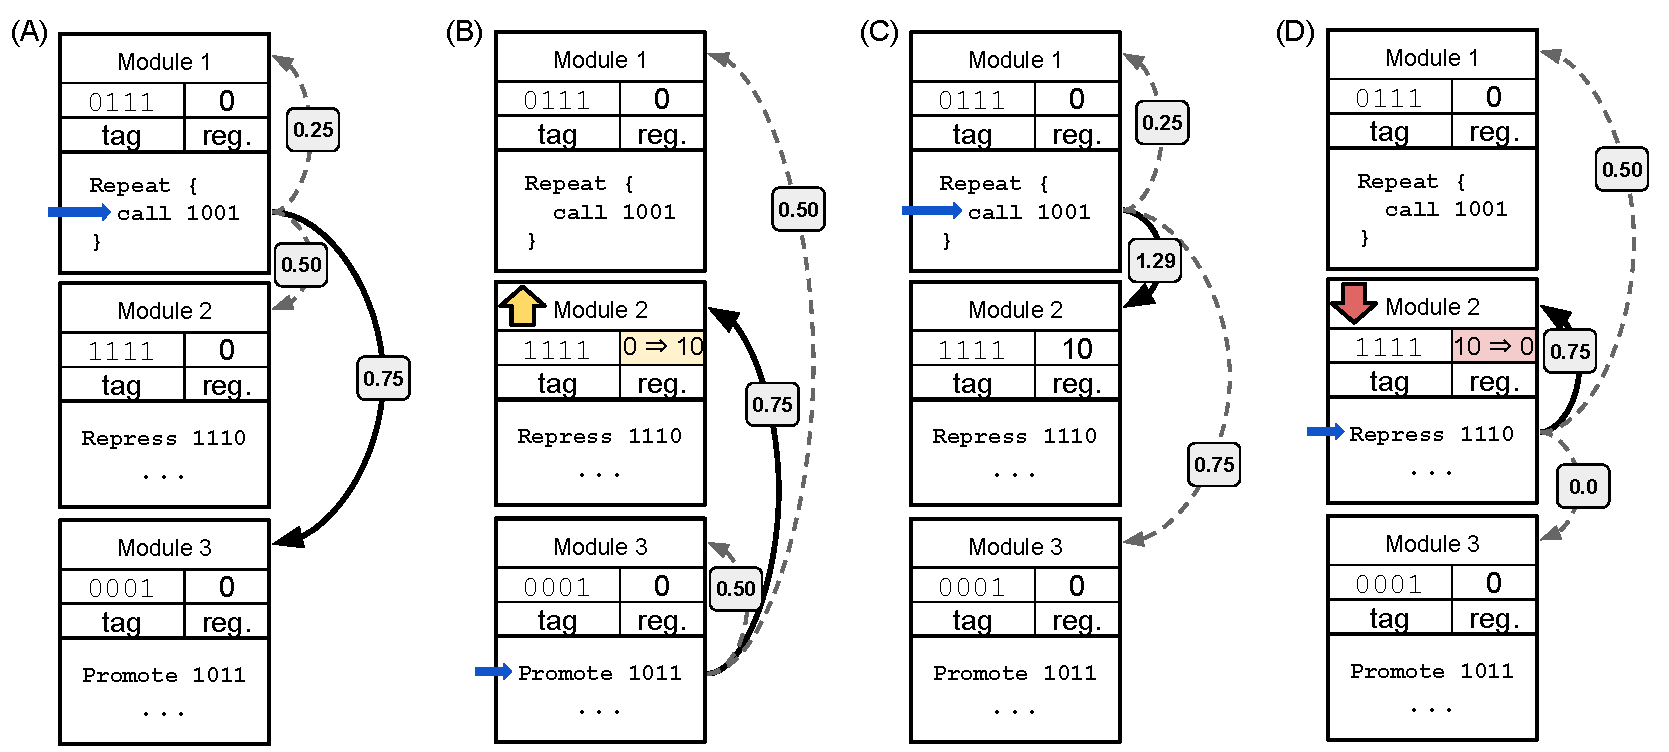
\includegraphics[width=\textwidth]{chapters/05-tag-based-genetic-regulation/media/regulation-example.pdf}
    \caption{\small
    \textbf{Tag-based genetic regulation example.}
    This example depicts a simple oscillating regulatory network instantiated using tag-based regulation.
    In this example, tags are length-4 bit strings. 
    The ``raw'' match score between two tags equals the number of matching bits between them.
    Regulation (reg.) modifies match scores for ``\code{call}'' instructions according to Equation \ref{chapter:tag-based-regulation:equ:reg-transform}.
    First (A), the \code{call 1001} in Module 1 executes, triggering Module 3. 
    Next (B), Module 3 is executed, promoting Module 2. 
    After Module 3 returns, the \code{call 1001} in Module 1 executes again (C); however, Module 2's promotion causes it to be triggered instead of Module 3. 
    Finally (D), Module 2 executes and represses itself, resetting its regulatory modifier to 0. 
    }
    \label{chapter:tag-based-regulation:fig:regulation-example}
\end{figure}
